%%%%%%%%%%%%%%%%%%%%%%%%%%%%%%%%%%%%%%%%%%%%%%%%%%%%%%%%%%%%%%%%%%%%%%
% Overleaf (WriteLaTeX) Example: Molecular Chemistry Presentation
%
% Source: http://www.overleaf.com
%
% In these slides we show how Overleaf can be used with standard 
% chemistry packages to easily create professional presentations.
% 
% Feel free to distribute this example, but please keep the referral
% to overleaf.com
% 
%%%%%%%%%%%%%%%%%%%%%%%%%%%%%%%%%%%%%%%%%%%%%%%%%%%%%%%%%%%%%%%%%%%%%%

\documentclass{beamer}

\mode<presentation>
{
  \usetheme{Madrid}       % or try default, Darmstadt, Warsaw, ...
  \usecolortheme{default} % or try albatross, beaver, crane, ...
  \usefonttheme{default}    % or try default, structurebold, ...
  \setbeamertemplate{navigation symbols}{}
  \setbeamertemplate{caption}[numbered]
} 

\usepackage[english]{babel}
\usepackage[utf8x]{inputenc}
\usepackage{chemfig}
\usepackage[version=3]{mhchem}

\usepackage{hyperref}
  \hypersetup{colorlinks=true}
  \hypersetup{urlcolor=blue}
  \hypersetup{linkcolor = .}
\usepackage{xcolor}
\usepackage{siunitx}
  \sisetup{separate-uncertainty = true}
\usepackage{physics}
\usepackage[font=small,labelfont=bf]{caption}
\usepackage{subcaption}
\usepackage[en-GB]{datetime2}
\usepackage{overpic}
\usepackage{feynmp}
\DeclareGraphicsRule{*}{mps}{*}{}

\usepackage{scalerel}
\newcommand{\mylbrace}[2]{\vspace{#2pt}\hspace{6pt}\scaleleftright[\dimexpr5pt+#1\dimexpr0.06pt]{\lbrace}{\rule[\dimexpr2pt-#1\dimexpr0.5pt]{-4pt}{#1pt}}{.}}
\newcommand{\myrbrace}[2]{\vspace{#2pt}\scaleleftright[\dimexpr5pt+#1\dimexpr0.06pt]{.}{\rule[\dimexpr2pt-#1\dimexpr0.5pt]{-4pt}{#1pt}}{\rbrace}\hspace{6pt}}

% Here's where the presentation starts, with the info for the title slide
\title[BESIII Oxford]{BESIII Oxford Group Meeting}
\author{Martin Tat}
\institute{Oxford LHCb}
\date{12th January 2022}

\titlegraphic{
\includegraphics[width = 4cm, height = 2.8cm]{lhcb.jpg}\hspace{1cm}~%
              
\includegraphics[width = 4cm, height = 2.8cm]{bes3.jpg}}

\begin{document}

\begin{frame}
  \titlepage
\end{frame}

% These three lines create an automatically generated table of contents.
%\begin{frame}{Outline}
%  \tableofcontents
%\end{frame}

\section{Double tag fit}

\begin{frame}{Double tag fit of $K\pi$}
  \begin{figure}
    \centering
    \begin{subfigure}{0.49\textwidth}
      \centering
      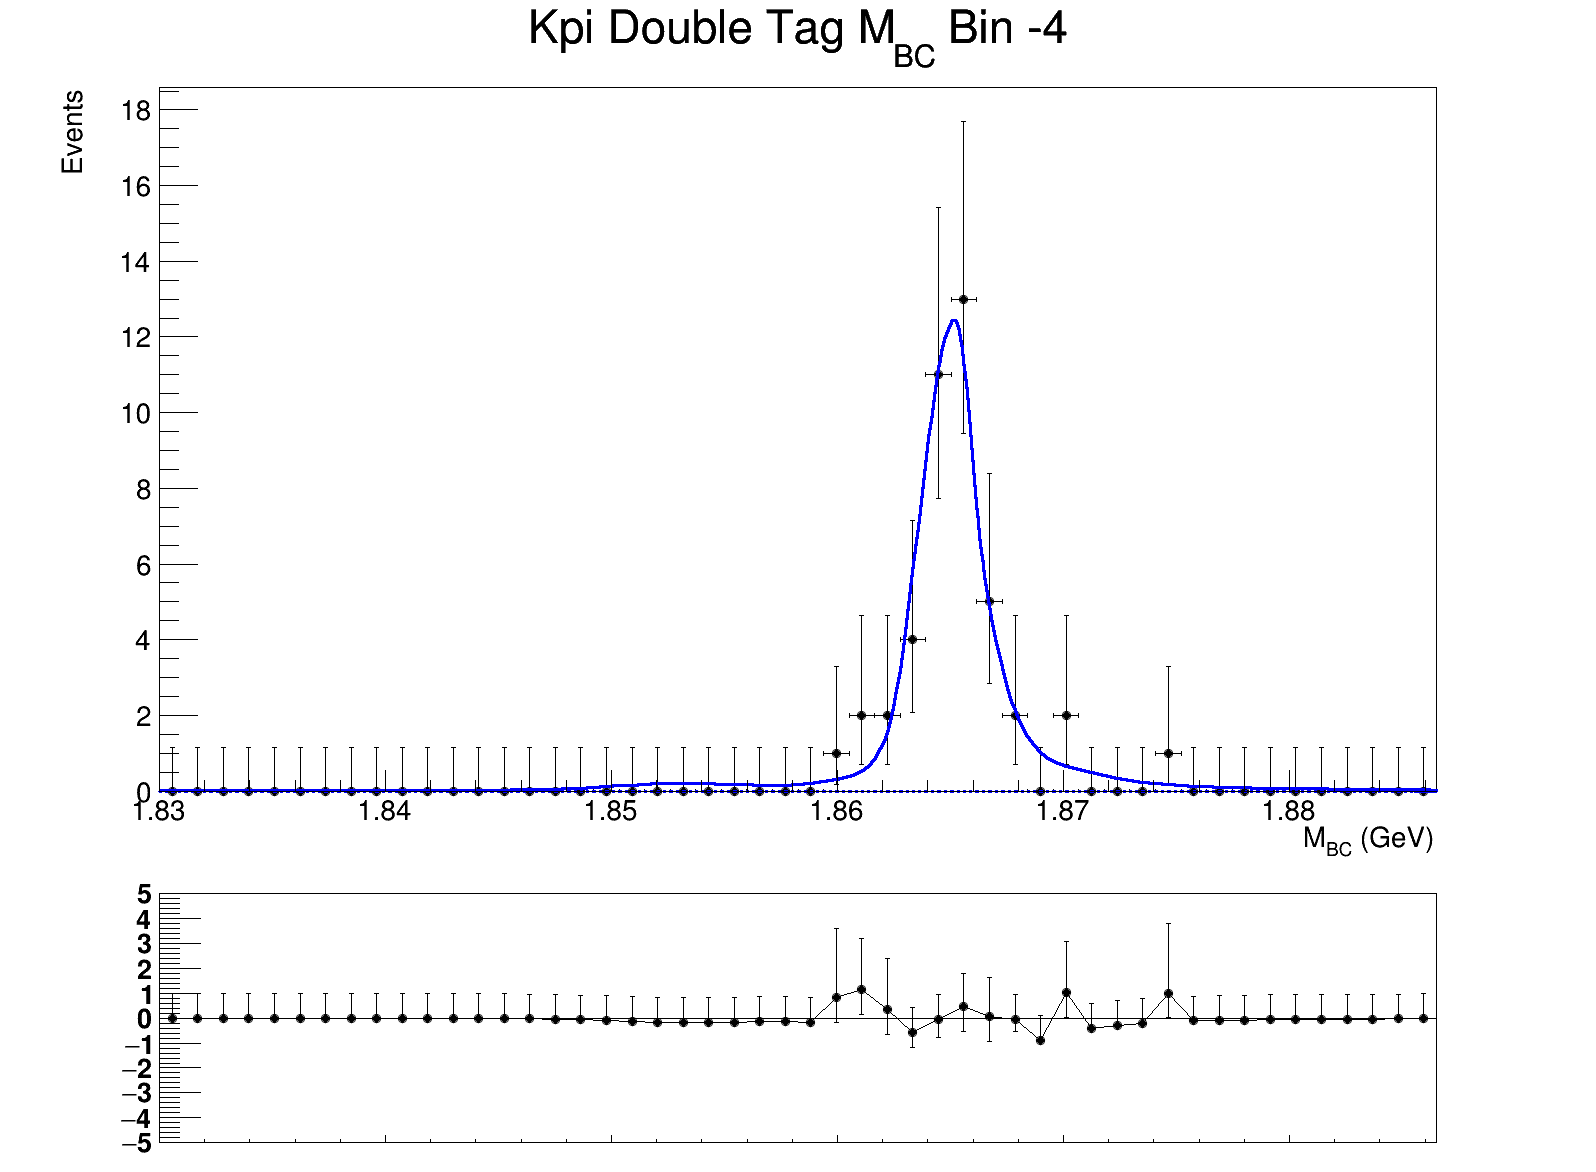
\includegraphics[width=\textwidth]{Plots/DoubleTagYield_DoubleTag_Flavour_KKpipi_vs_Kpi_SignalBinM4_TagBin0_old.png}
      \caption{Before bug fix}
    \end{subfigure}%
    \begin{subfigure}{0.49\textwidth}
      \centering
      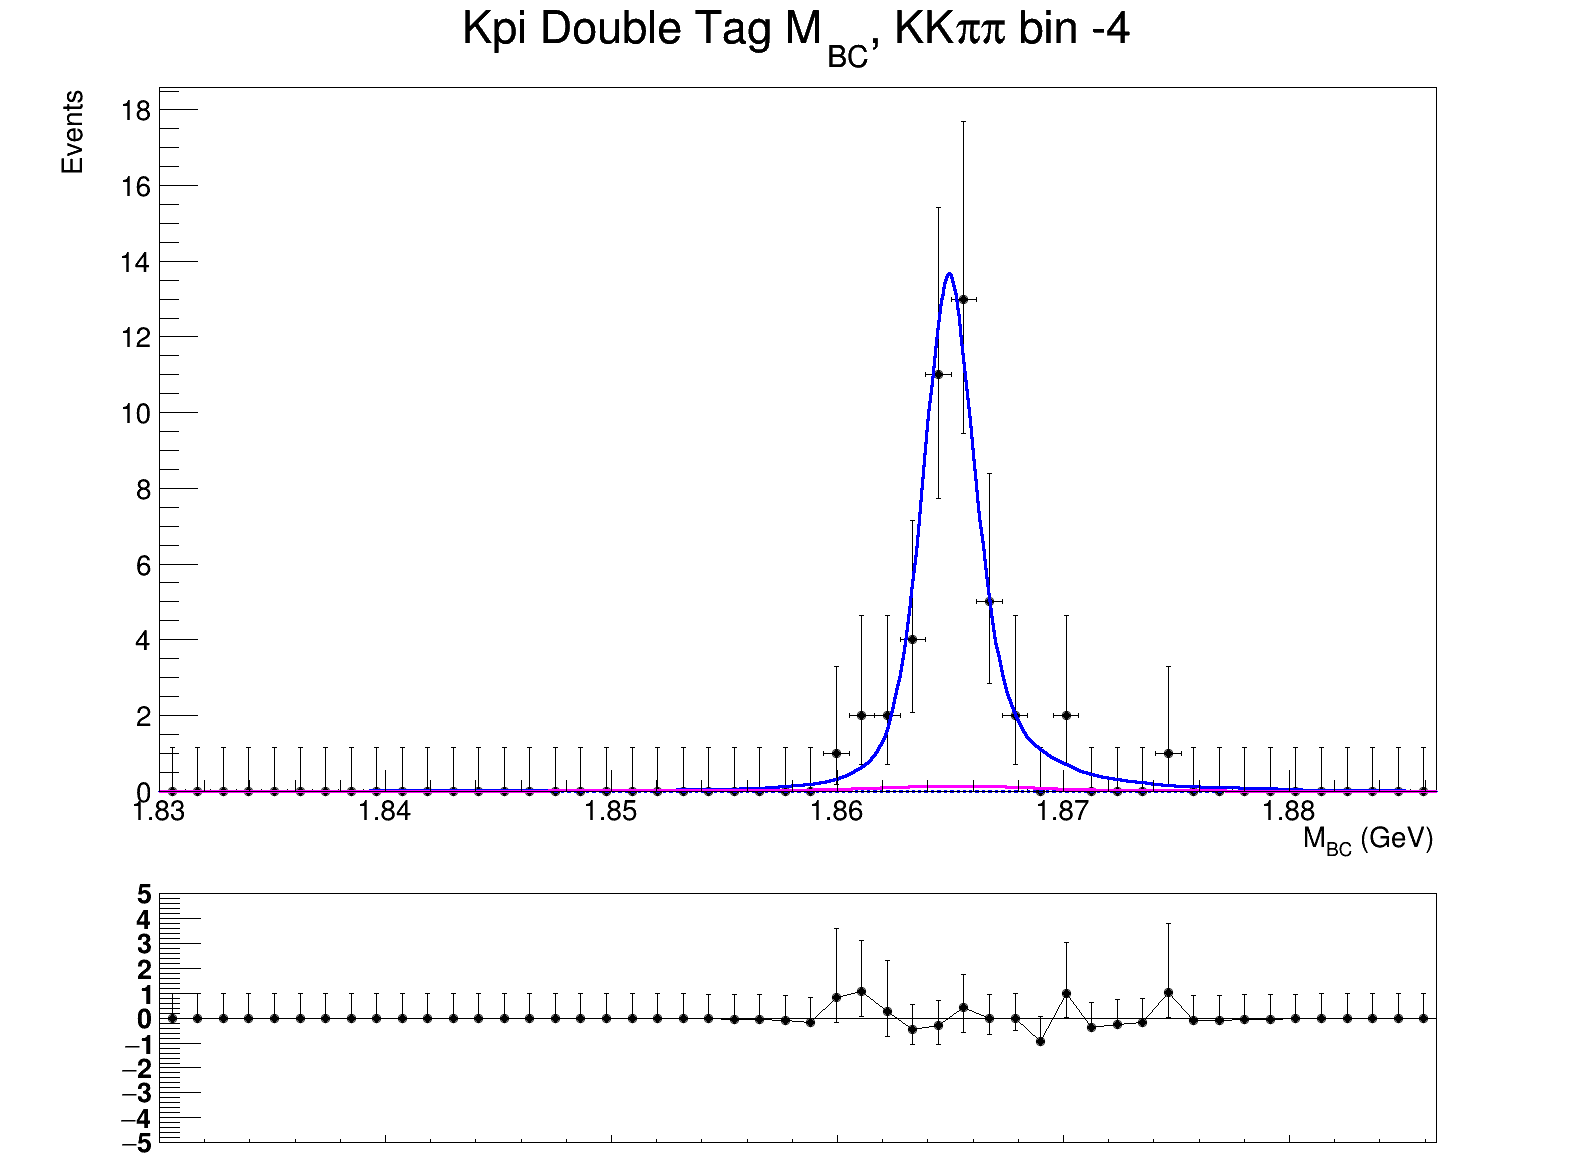
\includegraphics[width=\textwidth]{Plots/DoubleTagYield_DoubleTag_Flavour_KKpipi_vs_Kpi_SignalBinM4_TagBin0.png}
      \caption{After bug fix}
    \end{subfigure}
  \end{figure}
\end{frame}

\section{Efficiency corrections}
\begin{frame}{Efficiency corrections}
  \begin{itemize}
    \setlength\itemsep{1.5em}
    \item{Study bin migration}
    \item{Obtain resolution by comparing true and reconstructed momentum in signal MC}
    \item{Take a random event from signal MC, smear daughter momenta and determine ``Dalitz coordinate''}
  \end{itemize}
  \vspace{0.3cm}
  \begin{center}
    $\epsilon_{ij} = \frac{N^{\rm reconstructed}_{ij}}{N^{\rm generated}_j}$
  \end{center}
\end{frame}

\begin{frame}{Efficiency corrections}
  \begin{figure}
    \centering
    \begin{subfigure}{0.38\textwidth}
      \centering
      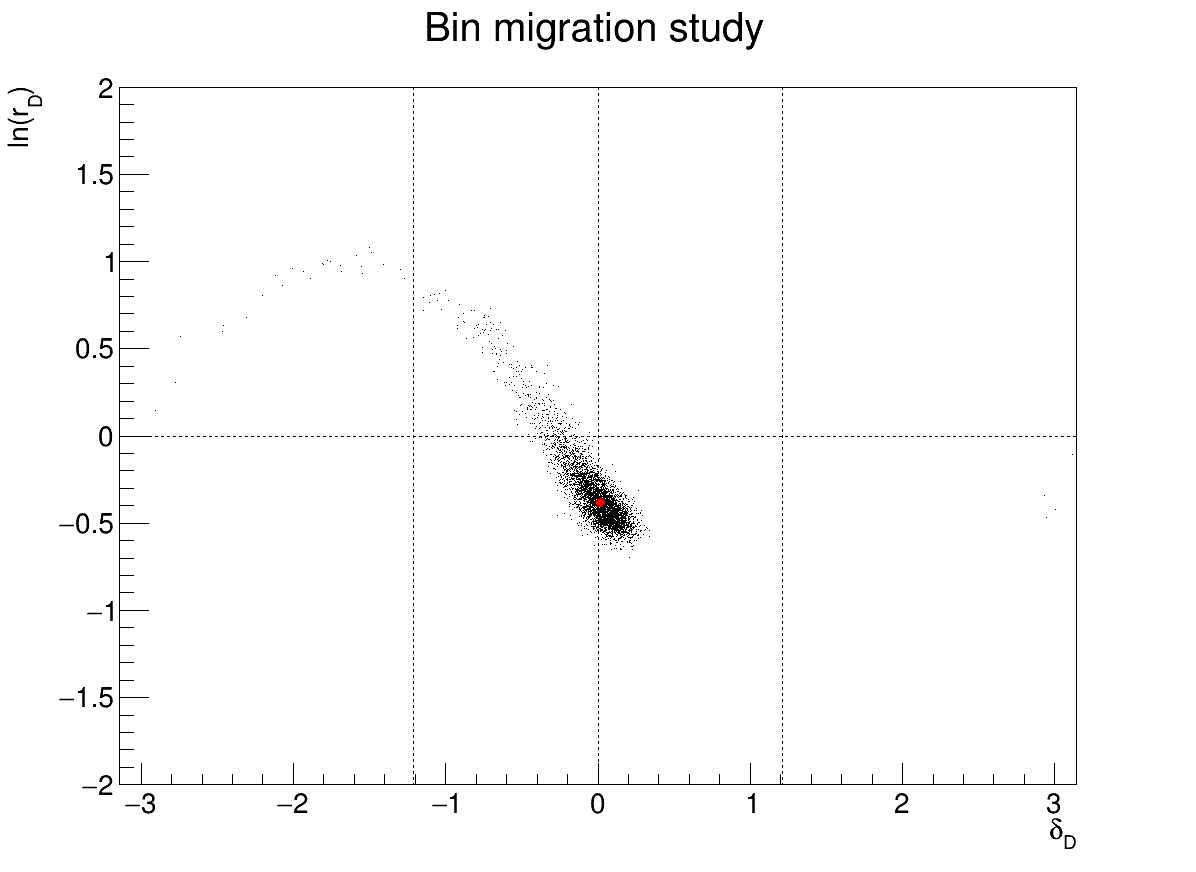
\includegraphics[width=\textwidth]{Plots/BinMigration_Point0.png}
    \end{subfigure}%
    \begin{subfigure}{0.38\textwidth}
      \centering
      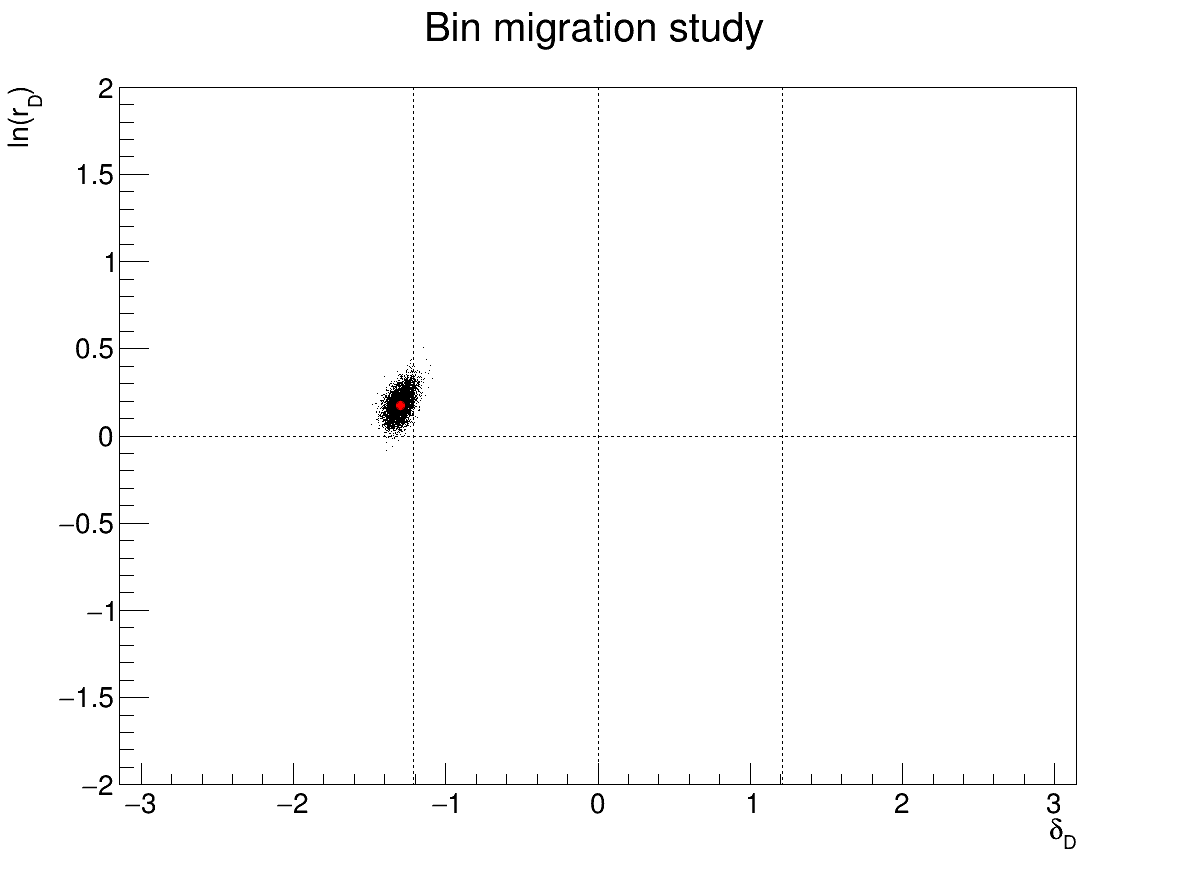
\includegraphics[width=\textwidth]{Plots/BinMigration_Point3.png}
    \end{subfigure}
    \begin{subfigure}{0.38\textwidth}
      \centering
      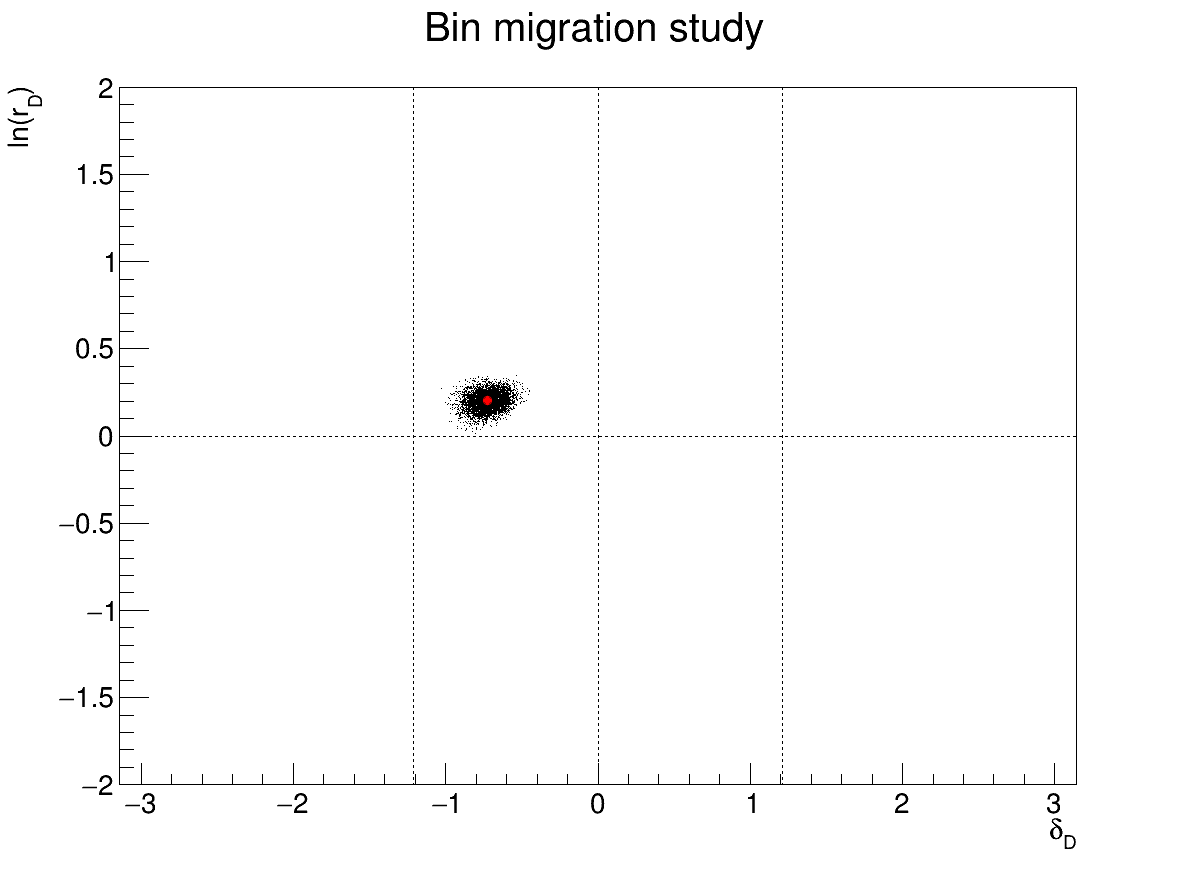
\includegraphics[width=\textwidth]{Plots/BinMigration_Point4.png}
    \end{subfigure}%
    \begin{subfigure}{0.38\textwidth}
      \centering
      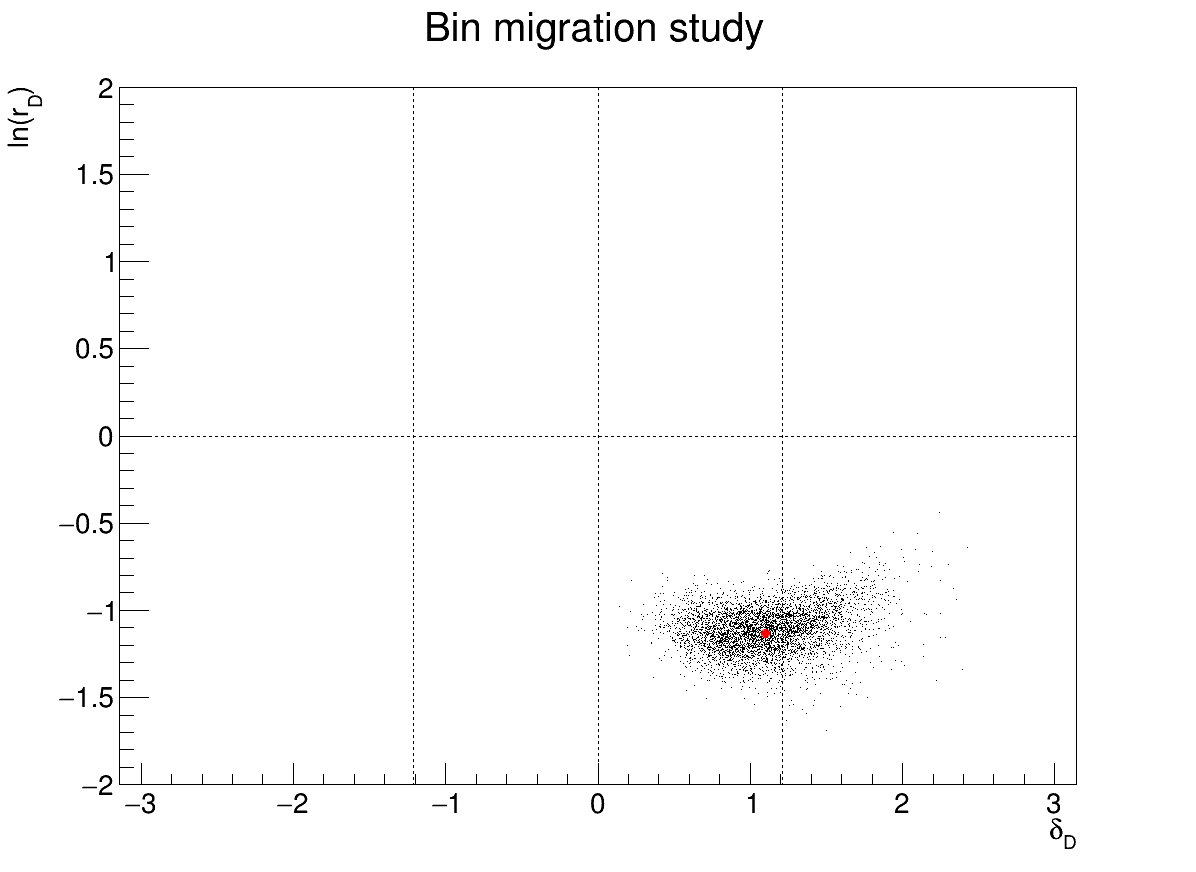
\includegraphics[width=\textwidth]{Plots/BinMigration_Point6.png}
    \end{subfigure}
  \end{figure}
\end{frame}

\begin{frame}{Efficiency corrections}
  \begin{figure}
    \centering
    \begin{subfigure}{0.38\textwidth}
      \centering
      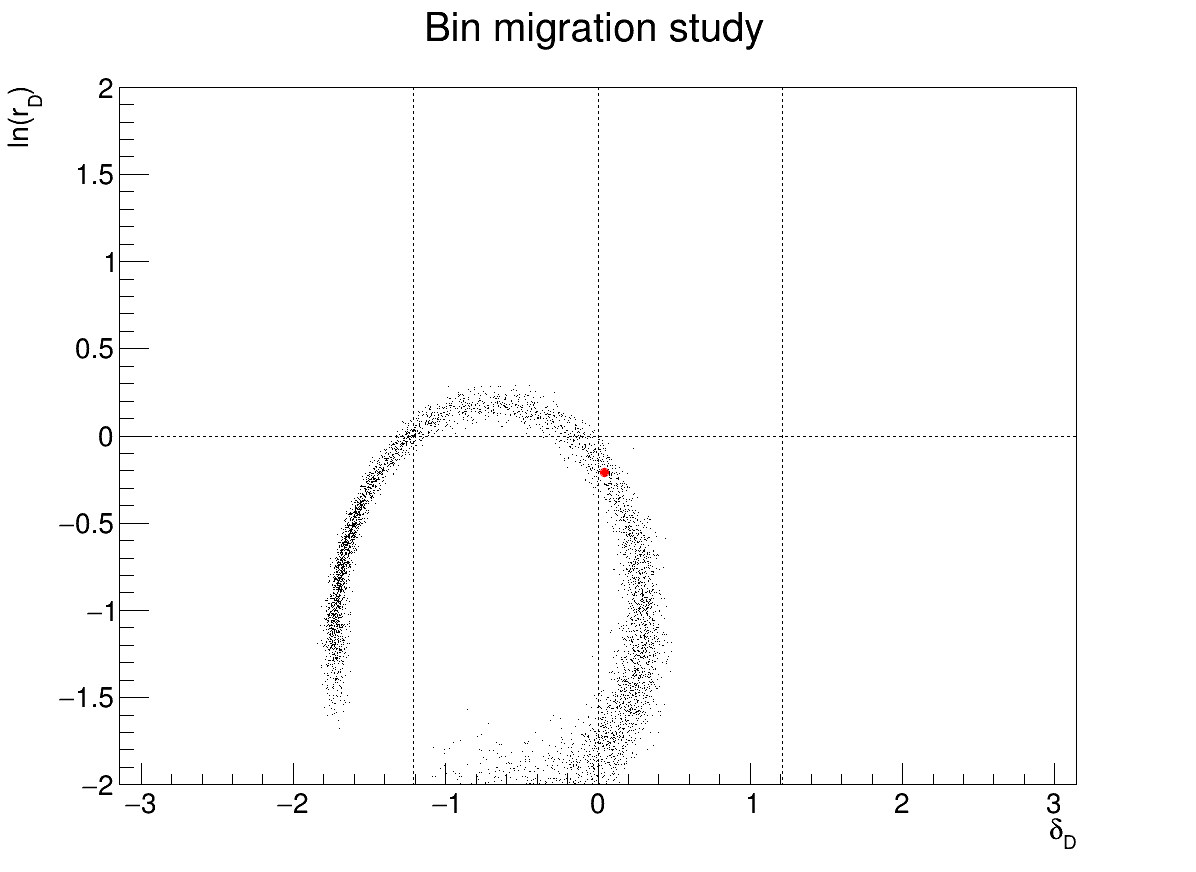
\includegraphics[width=\textwidth]{Plots/BinMigration_Point10.png}
    \end{subfigure}%
    \begin{subfigure}{0.38\textwidth}
      \centering
      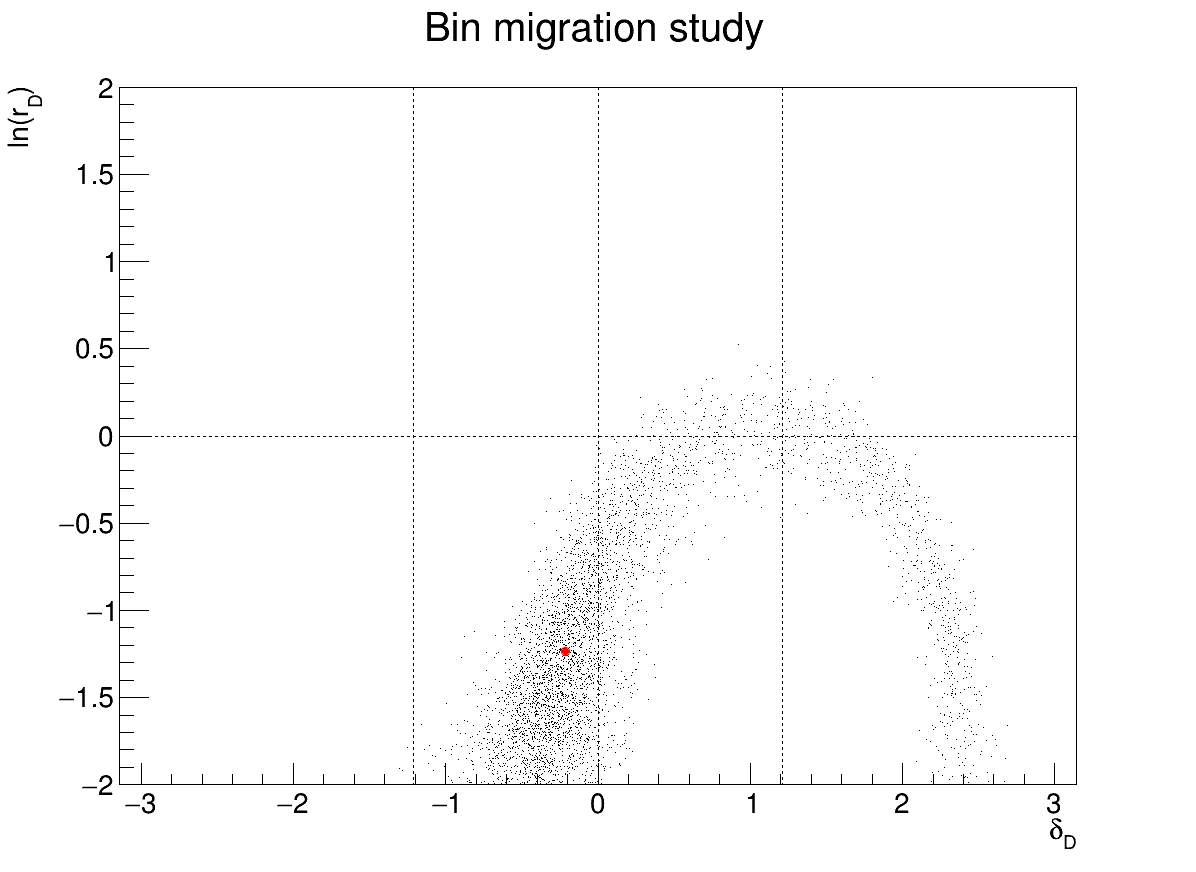
\includegraphics[width=\textwidth]{Plots/BinMigration_Point12.png}
    \end{subfigure}
    \begin{subfigure}{0.38\textwidth}
      \centering
      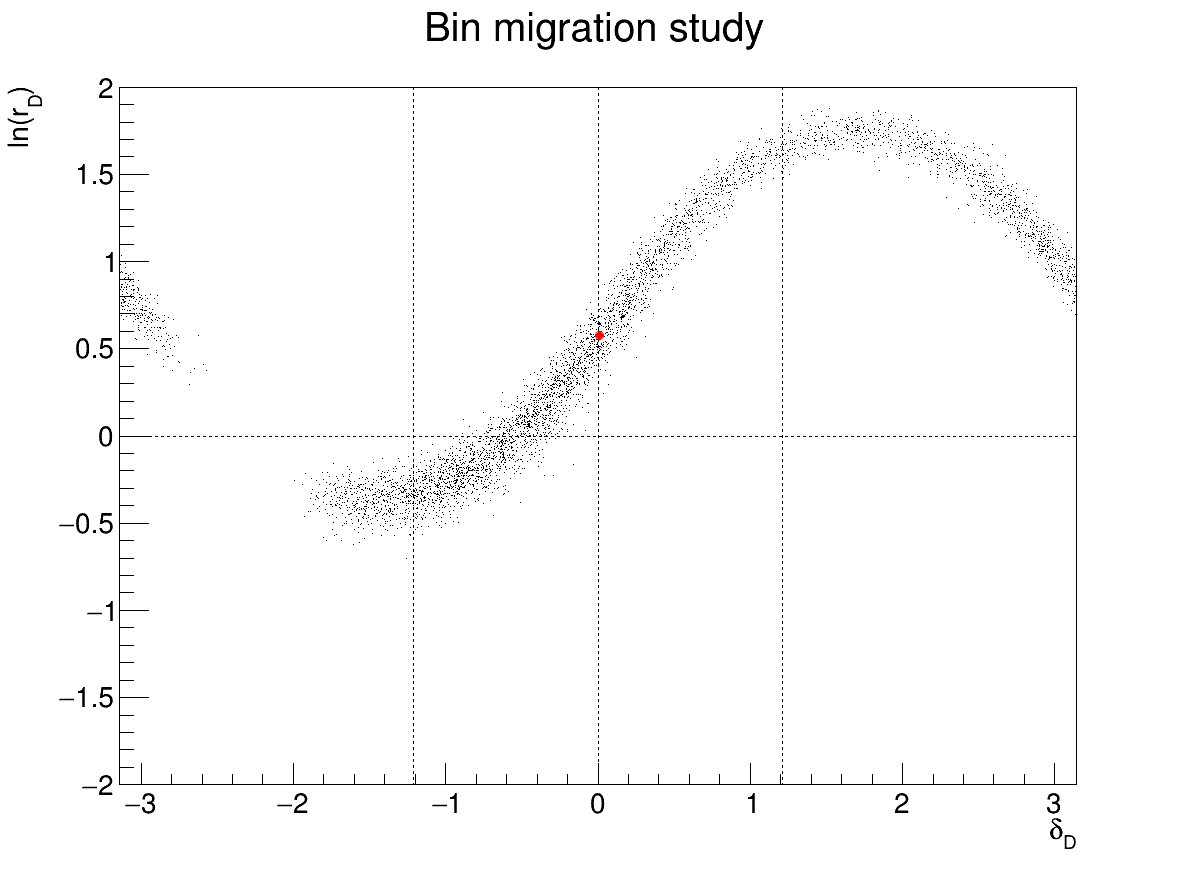
\includegraphics[width=\textwidth]{Plots/BinMigration_Point14.png}
    \end{subfigure}%
    \begin{subfigure}{0.38\textwidth}
      \centering
      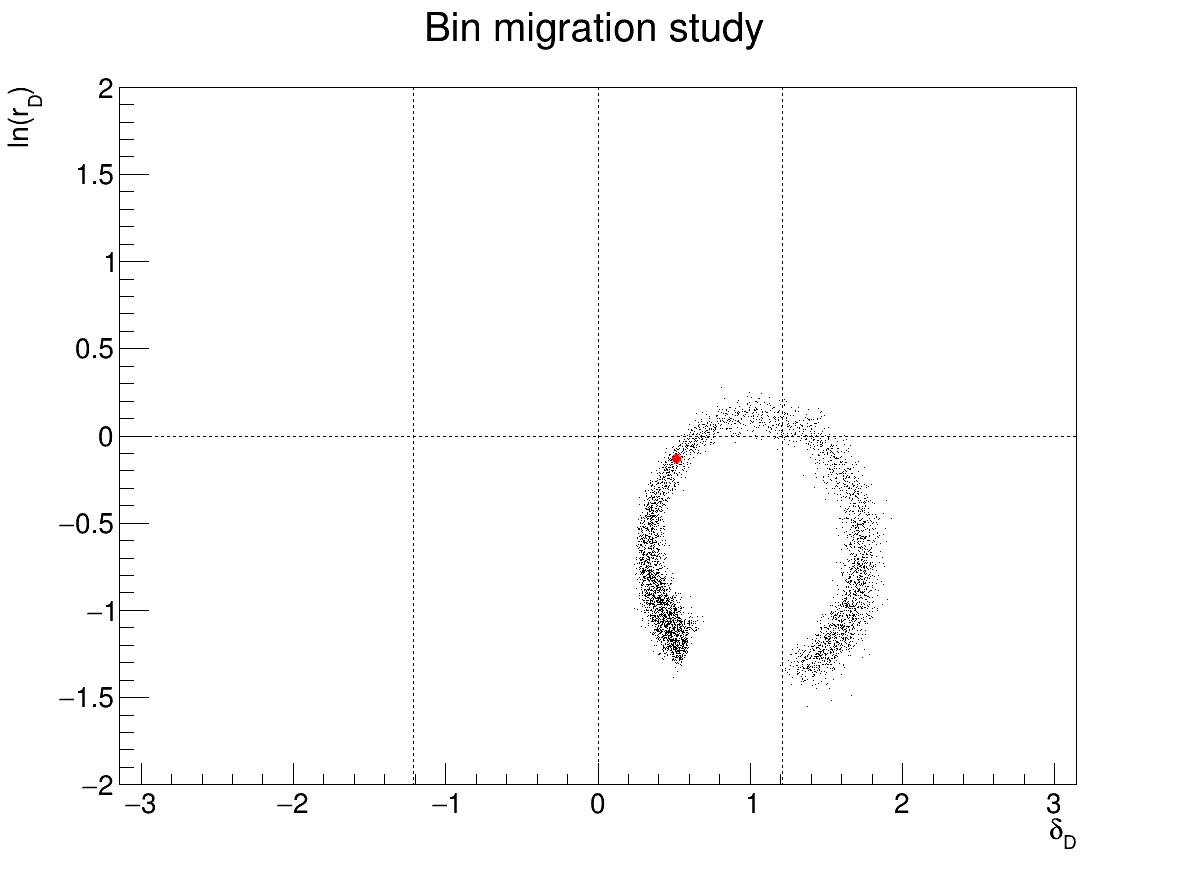
\includegraphics[width=\textwidth]{Plots/BinMigration_Point17.png}
    \end{subfigure}
  \end{figure}
\end{frame}

\section{DCS corrections}
\begin{frame}{DCS corrections}
  \begin{equation*}
    f_i = \frac{K_i}{K_i + K_{-i} - 2r_DR\big(c_i\cos(\delta_D) - s_i\sin(\delta_D)\big)}
  \end{equation*}
  \centering
  \def\arraystretch{1.2}%
  \begin{tabular}{c|ccc}
    Bin                         & $K\pi$               & $K\pi\pi^0$          & $K\pi\pi\pi$         \\
    \hline
    $R$                         & $\SI{1.0}{}$         & $\SI{0.79(4)}{}$     & $\SI{0.44(10)}{}$    \\
    $\delta_D(\si{\degree})$    & $\SI{190.0(42)}{}$   & $\SI{196(11)}{}$     & $\SI{161(28)}{}$     \\
    \hline
    $-4$                        & $\SI{1.0091(17)}{}$  & $\SI{1.0039(28)}{}$  & $\SI{1.0079(49)}{}$  \\
    $-3$                        & $\SI{0.9538(7)}{}$   & $\SI{0.9716(17)}{}$  & $\SI{0.9845(42)}{}$  \\
    $-2$                        & $\SI{0.9669(14)}{}$  & $\SI{0.9815(28)}{}$  & $\SI{0.9833(41)}{}$  \\
    $-1$                        & $\SI{1.0166(16)}{}$  & $\SI{1.0111(24)}{}$  & $\SI{1.0016(50)}{}$  \\
    $+1$                        & $\SI{1.0599(228)}{}$ & $\SI{1.0174(332)}{}$ & $\SI{1.0595(640)}{}$ \\
    $+2$                        & $\SI{0.7833(27)}{}$  & $\SI{0.8574(75)}{}$  & $\SI{0.9089(193)}{}$ \\
    $+3$                        & $\SI{0.8263(60)}{}$  & $\SI{0.8959(132)}{}$ & $\SI{0.9021(197)}{}$ \\
    $+4$                        & $\SI{1.1850(229)}{}$ & $\SI{1.1198(313)}{}$ & $\SI{0.9913(528)}{}$ \\
    \hline
  \end{tabular}
\end{frame}

\section{\texorpdfstring{$K_i$}{Ki} results for \texorpdfstring{$KK\pi\pi$}{KKpipi} vs \texorpdfstring{$K\pi$}{Kpi}}
\begin{frame}{$K_i$ results for $KK\pi\pi$ vs $K\pi$}
  \begin{figure}
    \centering
    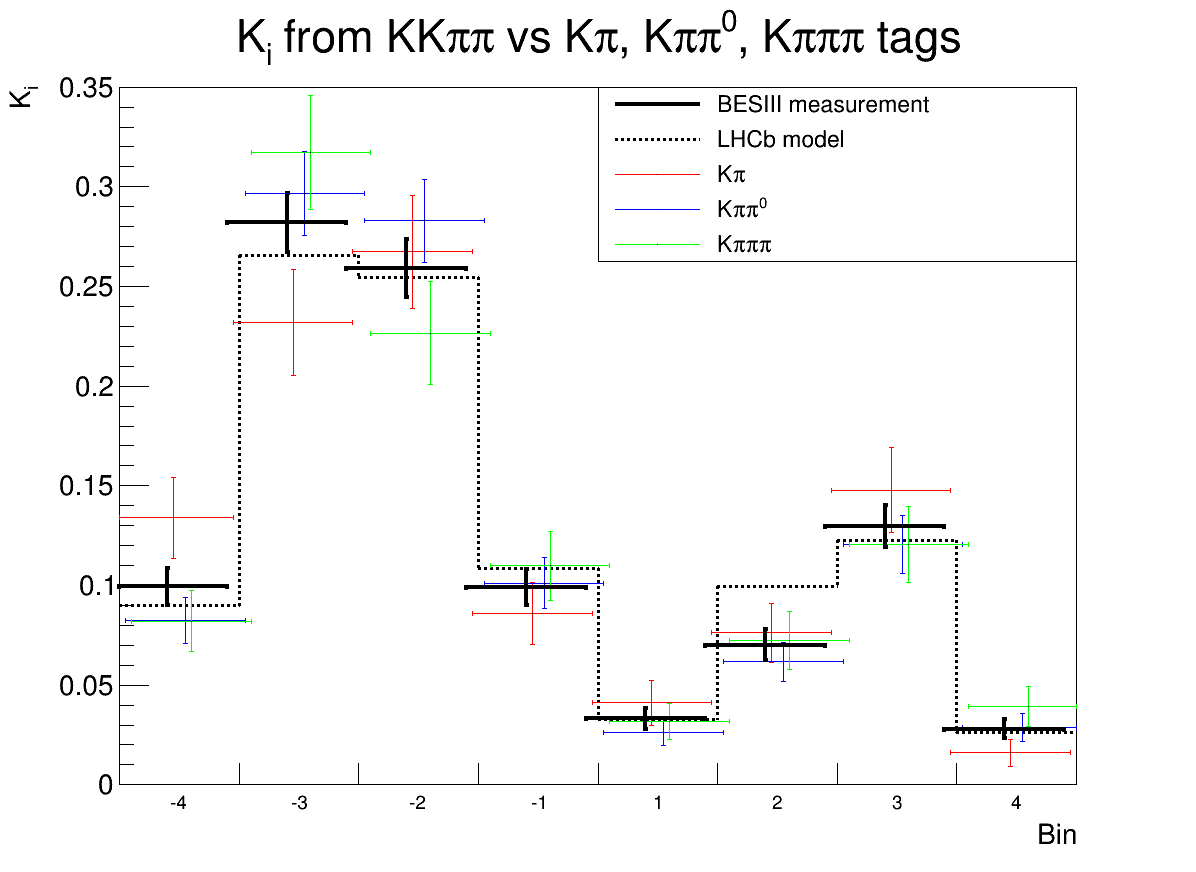
\includegraphics[width=0.9\textwidth]{Plots/Ki_Measured_vs_Model.png}
  \end{figure}
\end{frame}

\section{Measurement of \texorpdfstring{$F_+$}{F+}}
\begin{frame}{Measurement of $F_+$}
  \begin{figure}
    \centering
    \begin{subfigure}{0.38\textwidth}
      \centering
      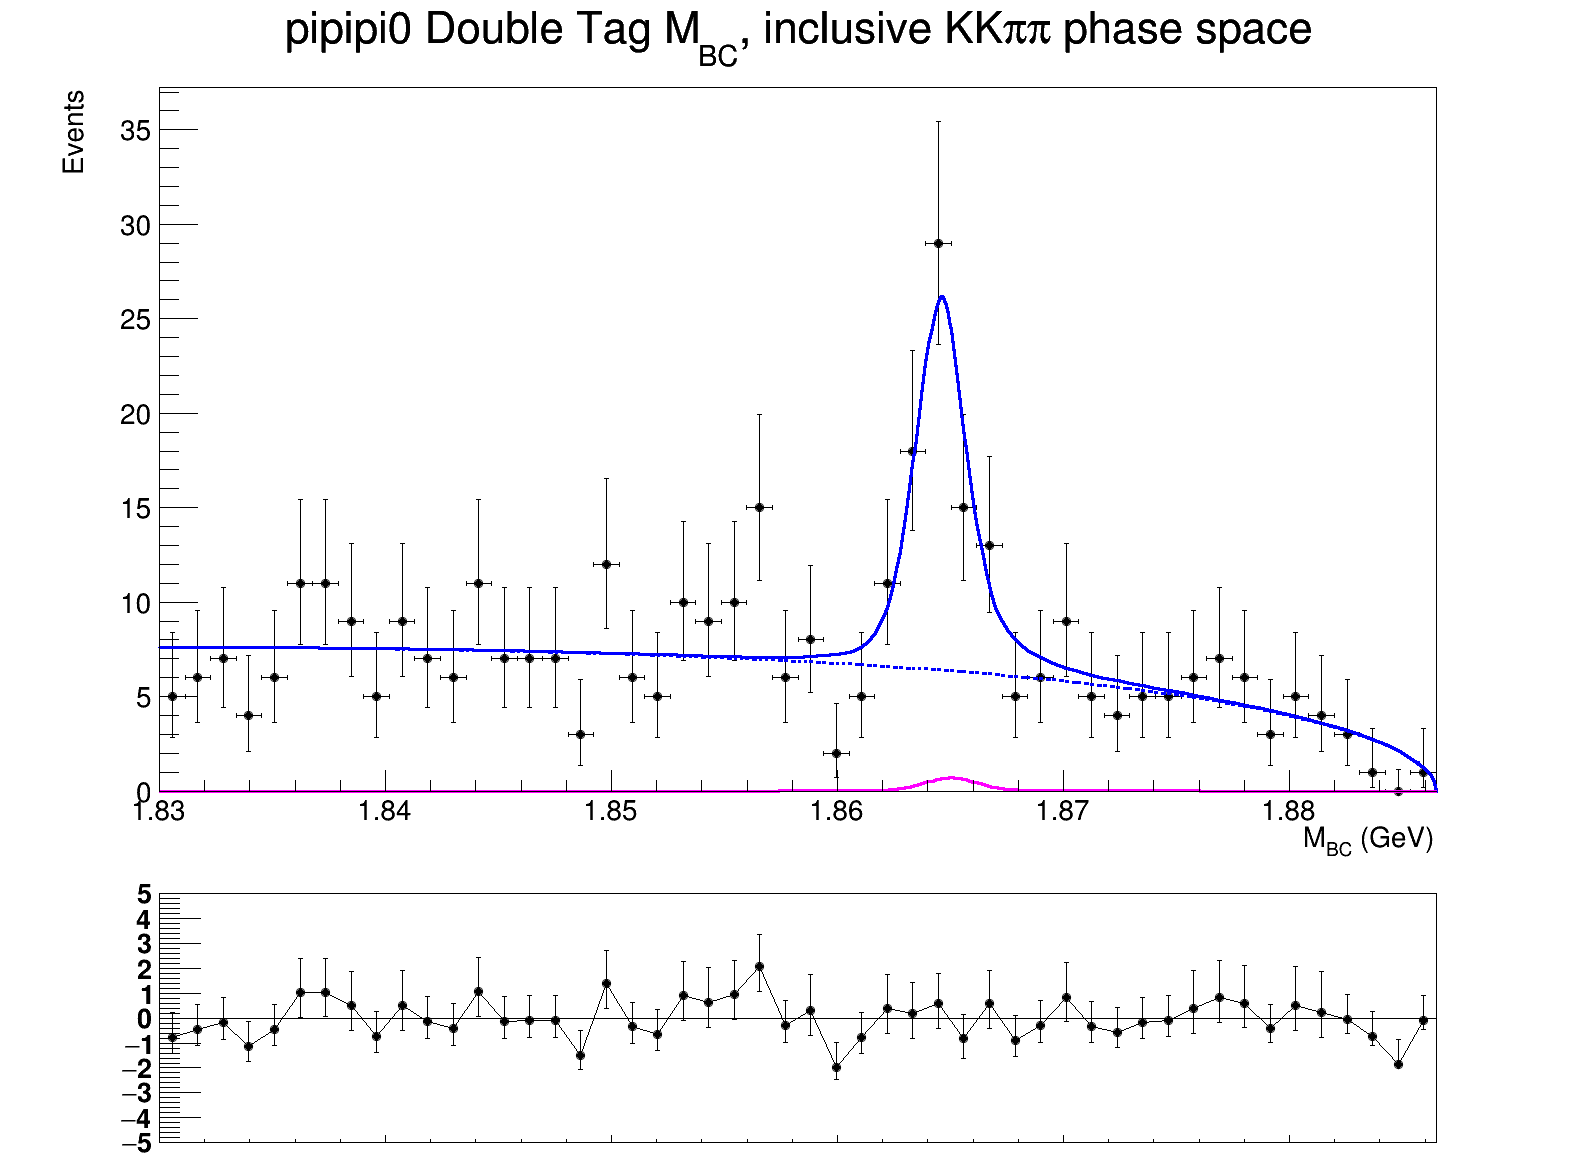
\includegraphics[width=\textwidth]{Plots/DoubleTagYield_DoubleTag_CP_KKpipi_vs_pipipi0_SignalBin0.png}
      \caption{$KK\pi\pi$ vs $\pi\pi\pi^0$}
    \end{subfigure}%
    \begin{subfigure}{0.38\textwidth}
      \centering
      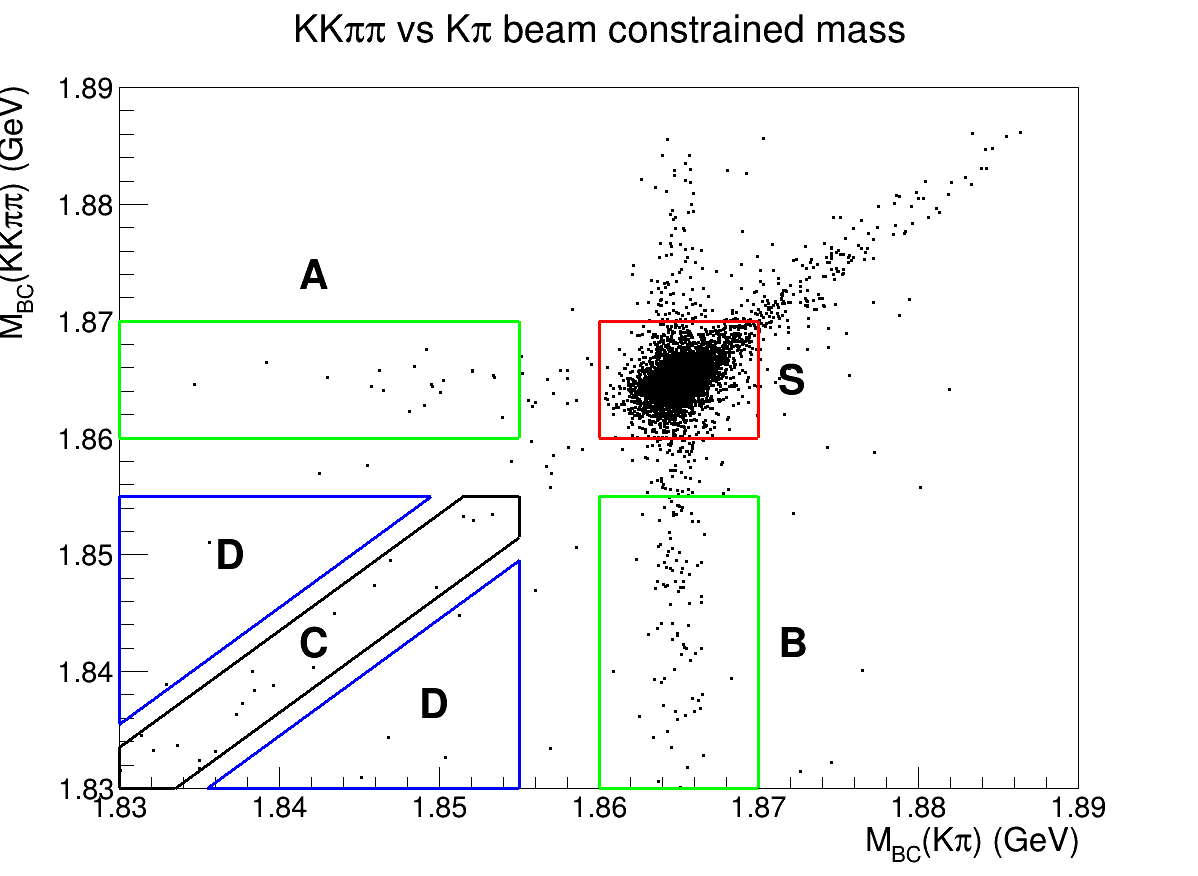
\includegraphics[width=\textwidth]{Plots/KpiDoubleTagYield.png}
      \caption{2D $m_{\rm BC}$}
    \end{subfigure}
  \end{figure}
  \begin{center}
    Cannot apply cut to $m_{\rm BC}^{\rm tag}$ because the sideband is removed \\
    Sideband subtraction for correctly reconstructed signal side?
  \end{center}
\end{frame}

\begin{frame}{Measurement of $F_+$}
  \begin{figure}
    \centering
    \begin{subfigure}{0.38\textwidth}
      \centering
      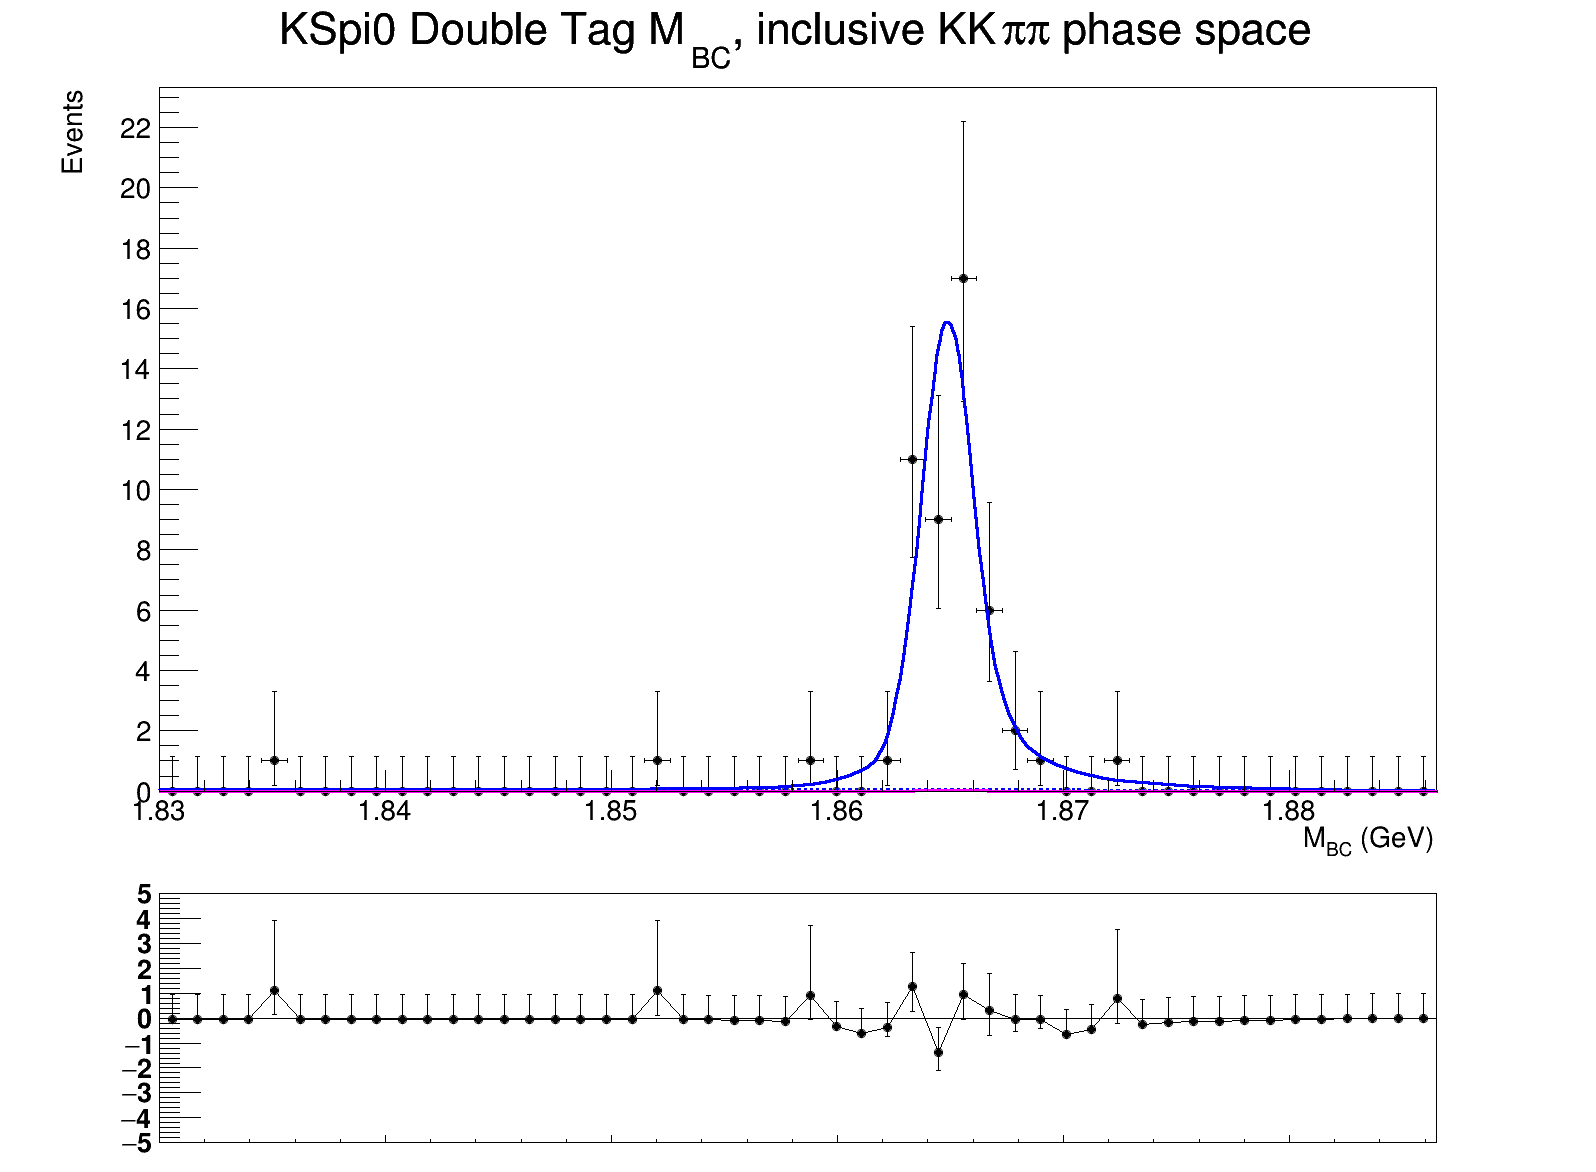
\includegraphics[width=\textwidth]{Plots/DoubleTagYield_DoubleTag_CP_KKpipi_vs_KSpi0_SignalBin0.png}
      \caption{$KK\pi\pi$ vs $K_S\pi^0$}
    \end{subfigure}%
    \begin{subfigure}{0.38\textwidth}
      \centering
      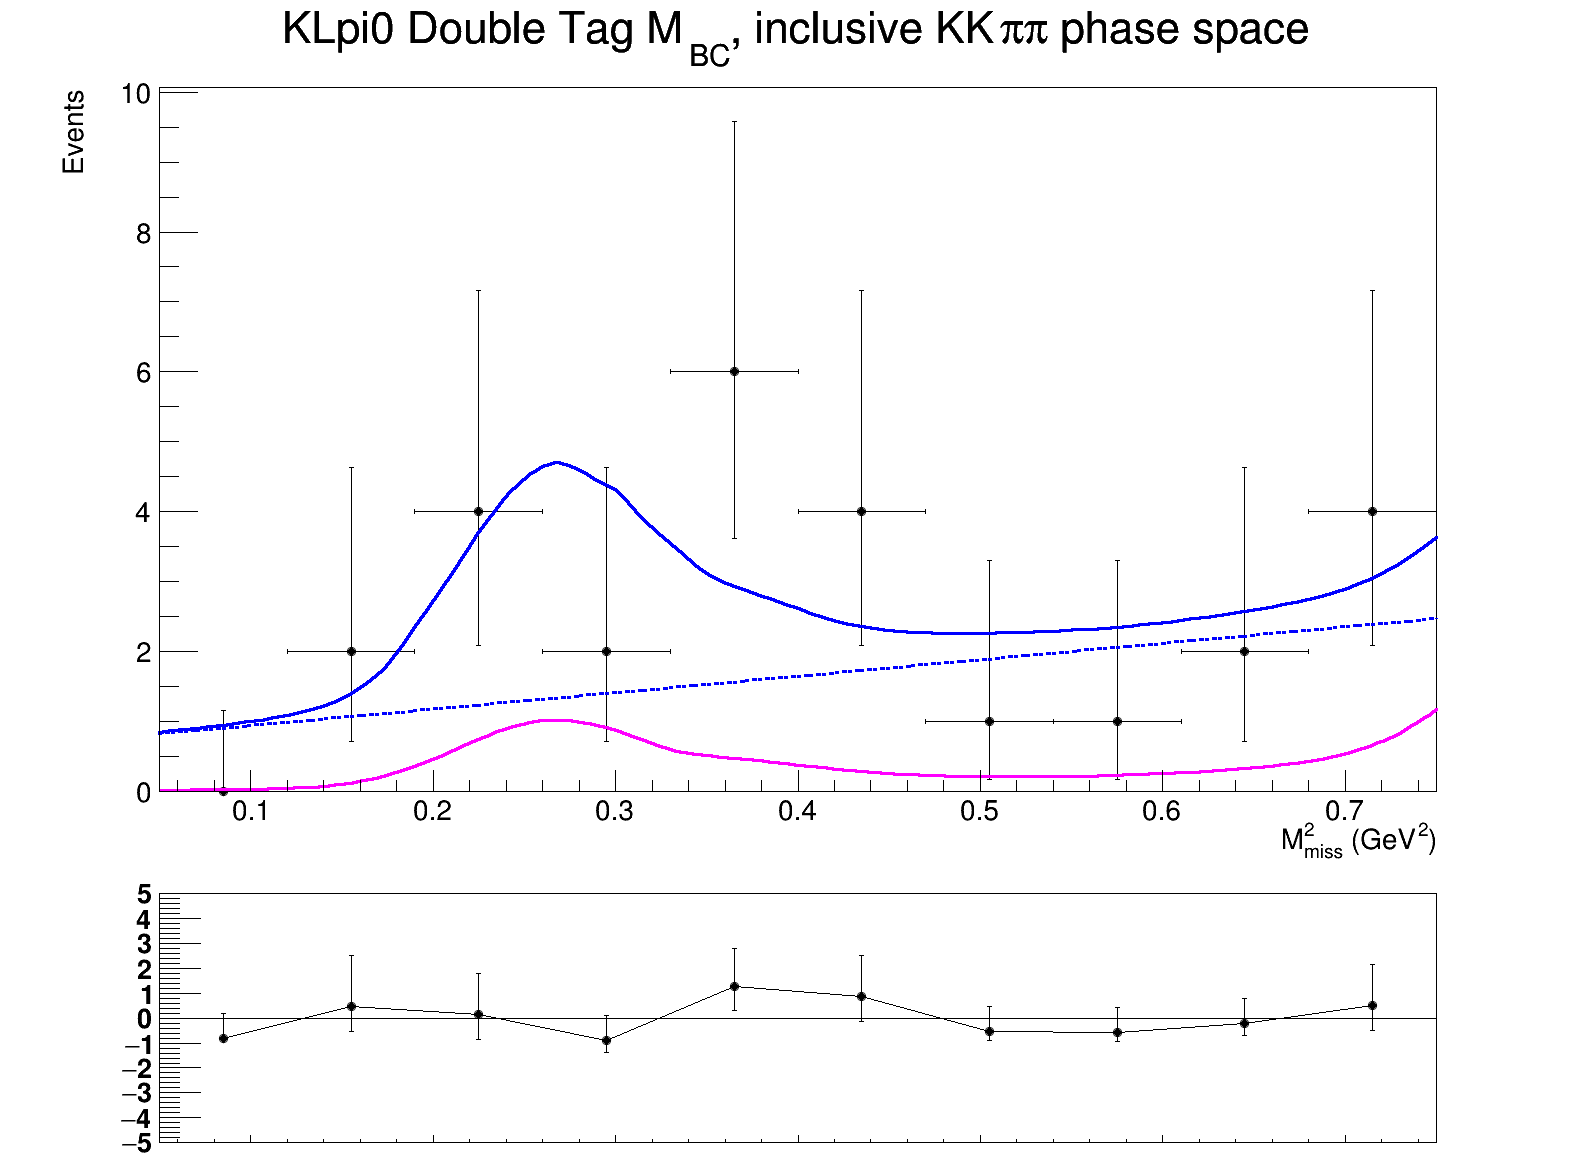
\includegraphics[width=\textwidth]{Plots/DoubleTagYield_DoubleTag_CP_KKpipi_vs_KLpi0_SignalBin0.png}
      \caption{$KK\pi\pi$ vs $K_Lpi^0$}
    \end{subfigure}
  \end{figure}
  \begin{center}
    Do the $K_L\pi^0$ plot look suspicious? \\
    How do I account for QC in $K_SKK$ backgrounds?
  \end{center}
\end{frame}

\begin{frame}{Measurement of $F_+$}
  \begin{figure}
    \centering
    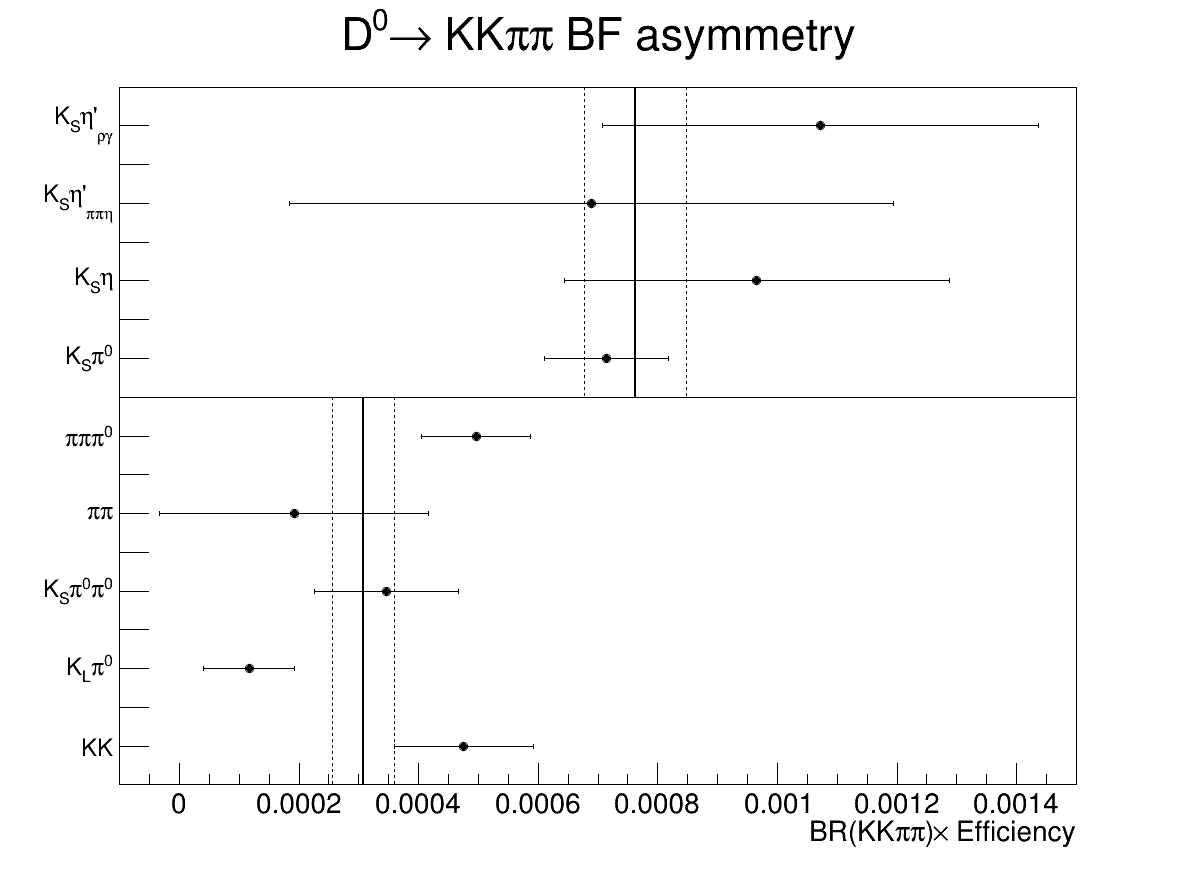
\includegraphics[width=0.9\textwidth]{Plots/CPeven_fraction_combination.png}
  \end{figure}
\end{frame}

\section{Some challanges with selection currently...}
\begin{frame}{Some challenges with selection currently...}
  \begin{enumerate}
    \setlength\itemsep{1.5em}
    \item{Very low tag efficiency for 4-body modes with kaons}
    \begin{itemize}
      \setlength\itemsep{1.0em}
      \item{Tracking efficiency is poor at low momentum}
      \item{Softer kaon momentum in $KK\pi\pi$}
      \item{How to loosen IP cuts?}
      \begin{itemize}
        \item{$V_{\rm xy} < \SI{1.0}{\centi\meter}$}
        \item{$V_{\rm z} < \SI{10.0}{\centi\meter}$}
      \end{itemize}
    \end{itemize}
    \item{Kalman kinematic fit in $K_Lh^+h^-$ gives very strange results}
    \begin{itemize}
      \setlength\itemsep{1.0em}
      \item{$K_LK^+K^-$ looks like it's working}
      \item{$K_L\pi^+\pi^-$ fit doesn't change pion momenta}
      \item{$\chi^2$ is too small ($10^{-6}$)}
    \end{itemize}
  \end{enumerate}
\end{frame}

\section{Next steps}
\begin{frame}{Conclusion and next steps}
  \begin{itemize}
    \setlength\itemsep{1.5em}
    \item{$K_i$ looks encouraging, can probably start some toy studies of binned CP double tags}
    \item{Bin migration seems large, but probably a result of binning scheme}
    \item{$F_+$ measurement looks possible with the current dataset}
    \item{Some issues with selection that requires more thinking...}
  \end{itemize}
\end{frame}

\end{document}
